
\section{Implementacija}

Razvijeni model optimizacije implementiran je u programskom jeziku \textbf{Python}, odabranom zbog čitljivosti, bogatog ekosustava biblioteka i široke primjene u znanstvenom računarstvu \cite{PythonSoftwareFoundation}. Python omogućuje brzu izradu prototipa, jednostavnu integraciju modula te učinkovitu obradu i vizualizaciju podataka.

\subsection{Korištene biblioteke}

Za izradu sustava korištene su sljedeće biblioteke (Tablica~\ref{tab:biblioteke}):

\begin{table}[H]
\centering
\caption{Korištene biblioteke u implementaciji}
\label{tab:biblioteke}
\begin{tabular}{|l|p{10cm}|}
\hline
\textbf{Biblioteka} & \textbf{Namjena} \\ \hline
NumPy & Numeričke operacije, generiranje slučajnih brojeva, vektorizacija izračuna. \\ \hline
SciPy & Statističke distribucije i znanstveno računarstvo; korišten za modeliranje PERT distribucije. \\ \hline
Matplotlib & Vizualizacija rezultata simulacija i optimizacijskih procesa. \\ \hline
DEAP & Implementacija genetskog algoritma, definiranje operatora selekcije, križanja i mutacije. \\ \hline
\end{tabular}
\end{table}

\subsection{Struktura sustava}


Sustav razvijen za potrebe ovog rada predstavlja cjeloviti eksperimentalni okvir dizajniran za analizu, kalibraciju i usporedbu optimizacijskih metodologija. Umjesto jednostavnog, monolitnog sustava, arhitektura je modularna i sastoji se od dva glavna analitička modula te jednog pomoćnog modula za obradu rezultata:

\begin{enumerate}
    \item \textbf{Modul za analizu i kalibraciju genetskog algoritma} \\
    Ovaj modul predstavlja temelj istraživanja i odgovara na pitanje: \emph{``Kako optimalno konfigurirati genetski algoritam za rješavanje zadanog problema?''}. Njegova primarna svrha je provođenje detaljne ablacijske studije (Ablation Study) kako bi se ispitao utjecaj svakog ključnog parametra na performanse algoritma.
    
    \textbf{Funkcionalnosti:}
    \begin{itemize}
        \item Sustavno testiranje različitih konfiguracija genetskog algoritma (standardni GA, bez križanja, bez mutacije, s povećanim brojem generacija, s većom populacijom).
        \item Višestruko pokretanje (\( \text{RUNS} = 10 \)) svake konfiguracije radi osiguravanja statističke značajnosti rezultata.
        \item Izračunavanje metrika performansi, uključujući prosječnu vrijednost (mean) i standardnu devijaciju (std) za ROI i procijenjeno trajanje.
        \item \textbf{Izlaz modula:} ``Šampionska'' konfiguracija – skup optimalnih parametara za genetski algoritam koji će se koristiti u daljnjoj analizi.
    \end{itemize}

    \item \textbf{Modul za usporednu analizu optimizacijskih scenarija} \\
    Ovaj modul čini srž diplomskog rada i koristi ``šampionsku'' konfiguraciju, definiranu u prethodnom modulu, za provođenje konačne usporedbe triju različitih pristupa rješavanju problema.
    
    \textbf{Funkcionalnosti:}
    \begin{itemize}
        \item Implementacija i izvršavanje triju ključnih scenarija:
        \begin{itemize}
            \item \textbf{Osnovni model (Random Search):} Slučajan odabir kao temeljna linija za usporedbu.
            \item \textbf{Klasični genetski algoritam:} Optimizacija usmjerena isključivo na maksimizaciju ROI-a.
            \item \textbf{Hibridni GA+MC model (NSGA-II):} Više-objektivna optimizacija koja istovremeno maksimizira ROI i minimizira rizik trajanja procijenjen Monte Carlo simulacijom.
        \end{itemize}
        \item Statistički robusna usporedba temeljem višestrukih pokretanja (\( \text{RUNS} = 10 \)) svakog scenarija.
        \item \textbf{Ulaz modula:} Optimalni parametri genetskog algoritma dobiveni iz Modula~1.
        \item \textbf{Izlaz modula:} Konačna tablica s usporednim rezultatima performansi (ROI, trajanje) i stabilnosti (standardna devijacija) za svaki od triju scenarija.
    \end{itemize}

    \item \textbf{Modul za obradu i vizualizaciju rezultata} \\
    Ovaj modul nije sekvencijalni korak, već pomoćni alat koji služi za interpretaciju rezultata dobivenih iz prva dva modula.
    
    \textbf{Funkcionalnosti:}
    \begin{itemize}
        \item Generiranje preglednih tablica s rezultatima pomoću \texttt{pandas} biblioteke.
        \item Spremanje rezultata u CSV format za daljnju analizu i dokumentaciju.
        \item (Potencijalno) stvaranje grafičkih prikaza, kao što su stupčasti dijagrami za usporedbu prosječnih vrijednosti ili 2D raspršeni dijagrami (scatter plots) za prikaz Paretovog fronta dobivenog iz NSGA-II algoritma.
    \end{itemize}
\end{enumerate}

\begin{figure}[H]
    \centering
    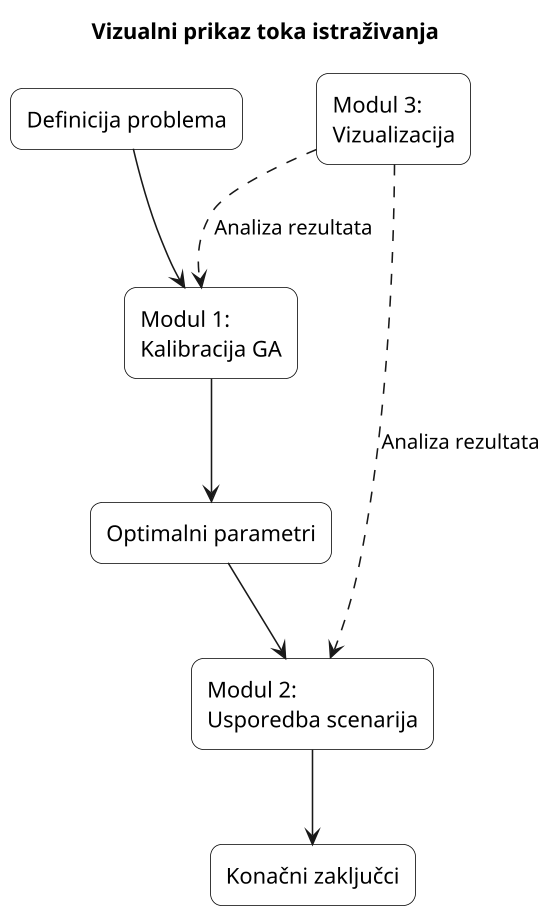
\includegraphics[width=0.9\textwidth]{slike/tijek_istrazivanja.png}
    \caption{Vizualni prikaz toka istraživanja}
    \label{tok istraživanja}
\end{figure}


\subsection{Monte Carlo simulacija}

Za svaki zadatak definirane su tri procjene trajanja: optimistična $(a)$, najvjerojatnija $(m)$ i pesimistična $(b)$.  
Distribucija trajanja modelirana je pomoću \textit{PERT distribucije} (Beta-PERT), gdje se očekivana vrijednost računa kao:

\[
\mu = \frac{a + 4m + b}{6}
\]

Parametri $\alpha_1$ i $\alpha_2$ Beta distribucije izračunavaju se prema \cite{Vose2008}:

\[
\alpha_1 = \frac{(\mu - a) \cdot (2m - a - b)}{(m - \mu)(b - a)}, \quad
\alpha_2 = \frac{\alpha_1 \cdot (b - \mu)}{(\mu - a)}
\]

Ako $\alpha_1 \leq 0$ ili $\alpha_2 \leq 0$, vrijednost se postavlja na $1.0$ radi numeričke stabilnosti.

\subsection{Genetski algoritam}

Implementacija genetskog algoritma provedena je pomoću biblioteke DEAP \cite{DEAP2012}.  
Svaki kromosom predstavlja potencijalni raspored aktivnosti, a optimizacija se temelji na višekriterijskoj funkciji pogodnosti koja uključuje:
\begin{itemize}
    \item trajanje projekta (na temelju Monte Carlo simulacije),
    \item troškove,
    \item dodatne projektne parametre.
\end{itemize}

Korišteni su sljedeći operatori:
\begin{itemize}
    \item \textbf{Selekcija:} turnirska i rulet-kolo selekcija,
    \item \textbf{Križanje:} PMX i OX1,
    \item \textbf{Mutacija:} zamjena pozicija gena (swap) i umetanje (insert).
\end{itemize}

\subsection{Vizualizacija}

Rezultati simulacija i optimizacije vizualizirani su pomoću \textbf{Matplotlib} \cite{Hunter2007} biblioteke kroz:
\begin{itemize}
    \item histograme distribucija trajanja zadataka,
    \item grafove konvergencije genetskog algoritma,
    \item usporedbe optimiziranih rješenja.
\end{itemize}


